\section{Текстовые строки}

\subsection{\CCpp}

\label{C_strings}
Обычные строки в Си заканчиваются нулем (\ac{ASCIIZ}-строки).

Причина, почему формат строки в Си именно такой (оканчивающийся нулем) вероятно историческая.
В [Dennis M. Ritchie, \IT{The Evolution of the Unix Time-sharing System}, (1979)]
мы можем прочитать:

\begin{framed}
\begin{quotation}
A minor difference was that the unit of I/O was the word, not the byte, because the PDP-7 was a word-addressed
machine. In practice this meant merely that all programs dealing with character streams ignored null
characters, because null was used to pad a file to an even number of characters.
\end{quotation}
\end{framed}

\myindex{Hiew}
Строки выглядят в Hiew или FAR Manager точно так же:

\begin{lstlisting}
int main()
{
	printf ("Hello, world!\n");
};
\end{lstlisting}

\begin{figure}[H]
\centering
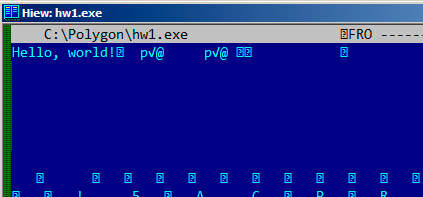
\includegraphics[scale=\NormalScale]{digging_into_code/strings/C-string.png}
\caption{Hiew}
\end{figure}

% FIXME видно \n в конце, потом пробел

\subsection{Borland Delphi}
\myindex{Pascal}
\myindex{Borland Delphi}
Когда кодируются строки в Pascal и Delphi, сама строка предваряется 8-битным или 32-битным значением, в котором закодирована длина строки.

Например:

\begin{lstlisting}[caption=Delphi]
CODE:00518AC8                 dd 19h
CODE:00518ACC aLoading___Plea db 'Loading... , please wait.',0

...

CODE:00518AFC                 dd 10h
CODE:00518B00 aPreparingRun__ db 'Preparing run...',0
\end{lstlisting}

\subsection{Unicode}

\myindex{Unicode}
Нередко уникодом называют все способы передачи символов, когда символ занимает 2 байта или 16 бит.
Это распространенная терминологическая ошибка.
Уникод --- это стандарт, присваивающий номер каждому символу многих письменностей мира, но не описывающий
способ кодирования.

\myindex{UTF-8}
\myindex{UTF-16LE}
Наиболее популярные способы кодирования: 
UTF-8 (наиболее часто используется в Интернете и *NIX-системах) и UTF-16LE (используется в Windows).

\subsubsection{UTF-8}

\myindex{UTF-8}
UTF-8 это один из очень удачных способов кодирования символов.
Все символы латиницы кодируются так же, как и в ASCII-кодировке, а символы, выходящие за пределы
ASCII-7-таблицы, кодируются несколькими байтами.
0 кодируется, как и прежде, нулевыми байтом, так что все стандартные
функции Си продолжают работать с UTF-8-строками так же как и с обычными строками.

Посмотрим, как символы из разных языков кодируются в UTF-8 и как это выглядит в FAR, в кодировке 437

\footnote{Пример и переводы на разные языки были взяты здесь: 
\url{http://go.yurichev.com/17304}}:

\begin{figure}[H]
\centering
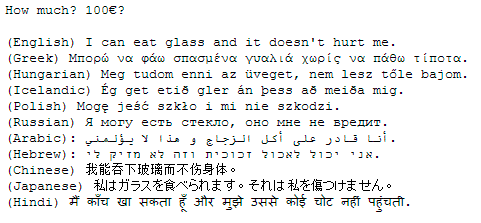
\includegraphics[scale=\NormalScale]{digging_into_code/strings/multilang_sampler.png}
\end{figure}

% FIXME: cut it
\begin{figure}[H]
\centering
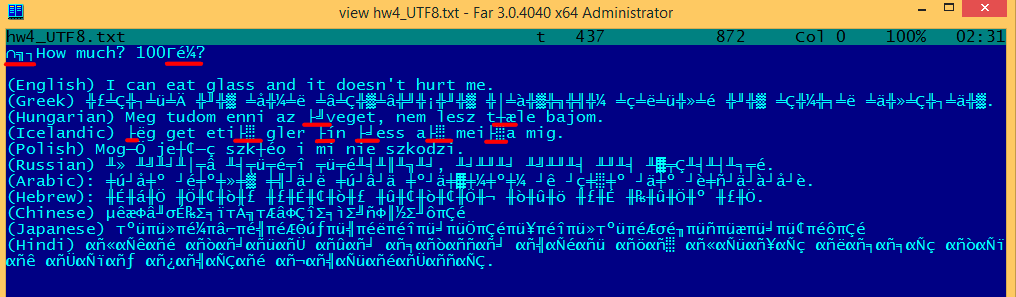
\includegraphics[scale=\FigScale]{digging_into_code/strings/multilang_sampler_UTF8.png}
\caption{FAR: UTF-8}
\end{figure}

Видно, что строка на английском языке выглядит точно так же, как и в ASCII-кодировке.
В венгерском языке используются латиница плюс латинские буквы с диакритическими знаками.
Здесь видно, что эти буквы кодируются несколькими байтами, они подчеркнуты красным.
То же самое с исландским и польским языками.
В самом начале имеется также символ валюты \q{Евро}, который кодируется тремя байтами.
Остальные системы письма здесь никак не связаны с латиницей.
По крайней мере о русском, арабском, иврите и хинди мы можем сказать, что здесь видны повторяющиеся
байты, что не удивительно, ведь, обычно буквы из одной и той же системы письменности расположены в одной
или нескольких таблицах уникода, поэтому часто их коды начинаются с одних и тех же цифр.

В самом начале, перед строкой \q{How much?}, видны три байта, которые на самом деле \ac{BOM}.
\ac{BOM} показывает, какой способ кодирования будет сейчас использоваться.

\subsubsection{UTF-16LE}

\myindex{UTF-16LE}
\myindex{Windows!Win32}
Многие функции win32 в Windows имееют суффикс \TT{-A} и \TT{-W}.
Первые функции работают с обычными строками, вторые с UTF-16LE-строками (\IT{wide}).
Во втором случае, каждый символ обычно хранится в 16-битной переменной типа \IT{short}.

Cтроки с латинскими буквами выглядят в Hiew или FAR как перемежающиеся с нулевыми байтами:

\begin{lstlisting}
int wmain()
{
	wprintf (L"Hello, world!\n");
};
\end{lstlisting}

\begin{figure}[H]
\centering
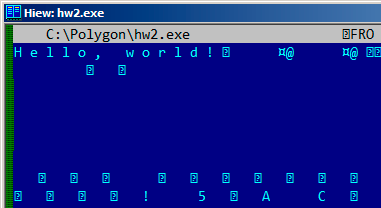
\includegraphics[scale=\NormalScale]{digging_into_code/strings/UTF16-string.png}
\caption{Hiew}
\end{figure}

Подобное можно часто увидеть в системных файлах \gls{Windows NT}:

\begin{figure}[H]
\centering
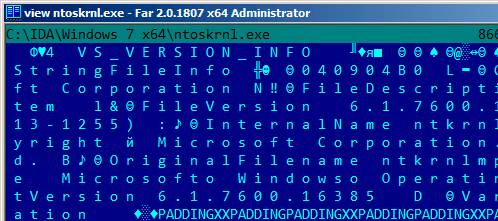
\includegraphics[scale=\NormalScale]{digging_into_code/strings/ntoskrnl_UTF16.png}
\caption{Hiew}
\end{figure}

\myindex{IDA}
В \IDA, уникодом называется именно строки с символами, занимающими 2 байта:

\begin{lstlisting}
.data:0040E000 aHelloWorld:
.data:0040E000                 unicode 0, <Hello, world!>
.data:0040E000                 dw 0Ah, 0
\end{lstlisting}

Вот как может выглядеть строка на русском языке (\q{И снова здравствуйте!}) закодированная в UTF-16LE:

\begin{figure}[H]
\centering
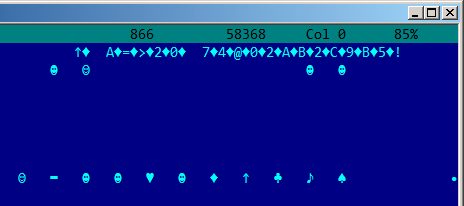
\includegraphics[scale=\NormalScale]{digging_into_code/strings/russian_UTF16.png}
\caption{Hiew: UTF-16LE}
\end{figure}

То что бросается в глаза\EMDASH{}это то что символы перемежаются ромбиками (который имеет код 4).
Действительно, в уникоде кирилличные символы находятся в четвертом блоке
\footnote{\href{http://go.yurichev.com/17003}{wikipedia}}.
Таким образом, все кирилличные символы в UTF-16LE находятся в диапазоне \TT{0x400-0x4FF}.

Вернемся к примеру, где одна и та же строка написана разными языками.
Здесь посмотрим в кодировке UTF-16LE.

% FIXME: cut it
\begin{figure}[H]
\centering
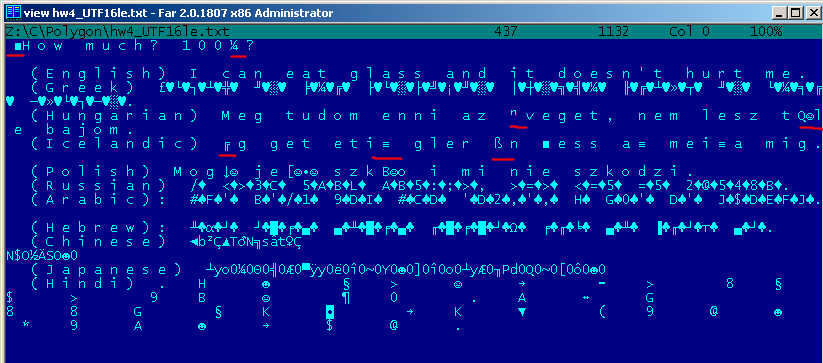
\includegraphics[scale=\FigScale]{digging_into_code/strings/multilang_sampler_UTF16.png}
\caption{FAR: UTF-16LE}
\end{figure}

Здесь мы также видим \ac{BOM} в самом начале.
Все латинские буквы перемежаются с нулевыми байтом.
Некоторые буквы с диакритическими знаками (венгерский и исландский языки) также подчеркнуты красным.

% TODO: strings *NIX utility. procmonitor also shows strings...

\subsection{Base64}
\myindex{Base64}

Кодировка base64 очень популярна в тех случаях, когда нужно передать двоичные данные как текстовую строку.

По сути, этот алгоритм кодирует 3 двоичных байта в 4 печатаемых символа:
все 26 букв латинского алфавита (в обоих регистрах), цифры, знак плюса (\q{+}) и слэша (\q{/}),
в итоге это получается 64 символа.

Одна отличительная особенность строк в формате base64, это то что они часто (хотя и не всегда) заканчиваются
одним или двумя символами знака равенства (\q{=}) для выравнивания (\gls{padding}), например:

\begin{lstlisting}
AVjbbVSVfcUMu1xvjaMgjNtueRwBbxnyJw8dpGnLW8ZW8aKG3v4Y0icuQT+qEJAp9lAOuWs=
\end{lstlisting}

\begin{lstlisting}
WVjbbVSVfcUMu1xvjaMgjNtueRwBbxnyJw8dpGnLW8ZW8aKG3v4Y0icuQT+qEJAp9lAOuQ==
\end{lstlisting}

Так что знак равенства (\q{=}) никогда не встречается в середине строк закодированных в base64.

